\documentclass[10pt,twocolumn,letterpaper]{article}

\usepackage{statcourse}
\usepackage{times}
\usepackage{epsfig}
\usepackage{graphicx}
\usepackage{amsmath}
\usepackage{amssymb}

% Include other packages here, before hyperref.

% If you comment hyperref and then uncomment it, you should delete
% egpaper.aux before re-running latex.  (Or just hit 'q' on the first latex
% run, let it finish, and you should be clear).
\usepackage[breaklinks=true,bookmarks=false]{hyperref}


\statcoursefinalcopy


\setcounter{page}{1}
\begin{document}


%%%%%%%%%%%%%%%%%%%%%%%%%%%%%%%%%%%%%%%%%%%%%%%%%%%%%%%%%%%%%%%
% DO NOT EDIT ANYTHING ABOVE THIS LINE
% EXCEPT IF YOU LIKE TO USE ADDITIONAL PACKAGES
%%%%%%%%%%%%%%%%%%%%%%%%%%%%%%%%%%%%%%%%%%%%%%%%%%%%%%%%%%%%%%%



%%%%%%%%% TITLE
\title{Arranging an Audio Track to other Genres\\
       by using CycleGAN-based Deep Learning Model 
       \thanks{Project proposal for Spring 2020, University of Wisconsin-Madison
               STAT453 Deep Learning course (Instructor: Sebastian Raschka);\\
               All authors contributed equally}
}

\author{Alex DongHyeon Seo\\
{\tt\small dseo22@wisc.edu}
\and
Hyecheol (Jerry) Jang\\
{\tt\small hyecheol.jang@wisc.edu}
\and
Stella Kim\\
{\tt\small ykim736@wisc.edu}
}

\maketitle
%\thispagestyle{empty}



% MAIN ARTICLE GOES BELOW
%%%%%%%%%%%%%%%%%%%%%%%%%%%%%%%%%%%%%%%%%%%%%%%%%%%%%%%%%%%%%%%


%%%%%%%%% ABSTRACT
\begin{abstract}
  Changing the genre of a song is one of the methods used when compositing music.
  To the best of our knowledge, musicians usually add their new ideas to the song,
  while trying to keep most of the special characteristics of the original song when arranging music.
  Similar to other artistic tasks that require human creativity,
  converting the genre of a song takes a significant amount of time and effort.
  In this project, we propose a method to translate a music genre by using machine-learning,
  which can generate a new song with comparably less amount of time than humans.
  Specifically, we utilized cycleGAN based model to translate a soundtrack to another soundtrack.\par
  Due to the complexity and difficulties of dealing with audio data,
  our model is able to handle files written with MIDI (Musical Instrument Digital Interface) specification only with
  specific characteristics.
  In the near future,
  we expect to expand our project to use regular audio files rather than MIDI to do our tasks to generalize our model.
  By doing so, we hope our model to be used for the general public without further modifications.
\end{abstract}

%%%%%%%%% BODY TEXT
\section{Introduction}

In this project, our goal is to change the genre of a music track, given a set of user inputs 
containing song and the desired genre. To accomplish the goal, the main model that we are going to 
consider is CycleGAN~\cite{zhu2017unpaired}-based model. Though Isola et al. proposed this 
architecture for unpaired Image-to-Image translation, we are hoping that this model with a proper
modification of the structure would accept relative information from audio tracks.

\section{Related Work}

Related work should be discussed here. This is an example of a citation \cite{mirjalili2018gender}. To format the citations properly, put the
corresponding references into the bibliography.bib file. You can obtain
BibTeX-formatted references for the "bib" file from Google Scholar 
(\url{https://scholar.google.com}), for example, by clicking on the 
double-quote character under a citation and then selecting \mbox{"BibTeX"} as
shown in Figure \ref{fig:google-scholar-1col} and 
Figure \ref{fig:google-scholar-2col}.

\begin{figure}[t]
\begin{center}
   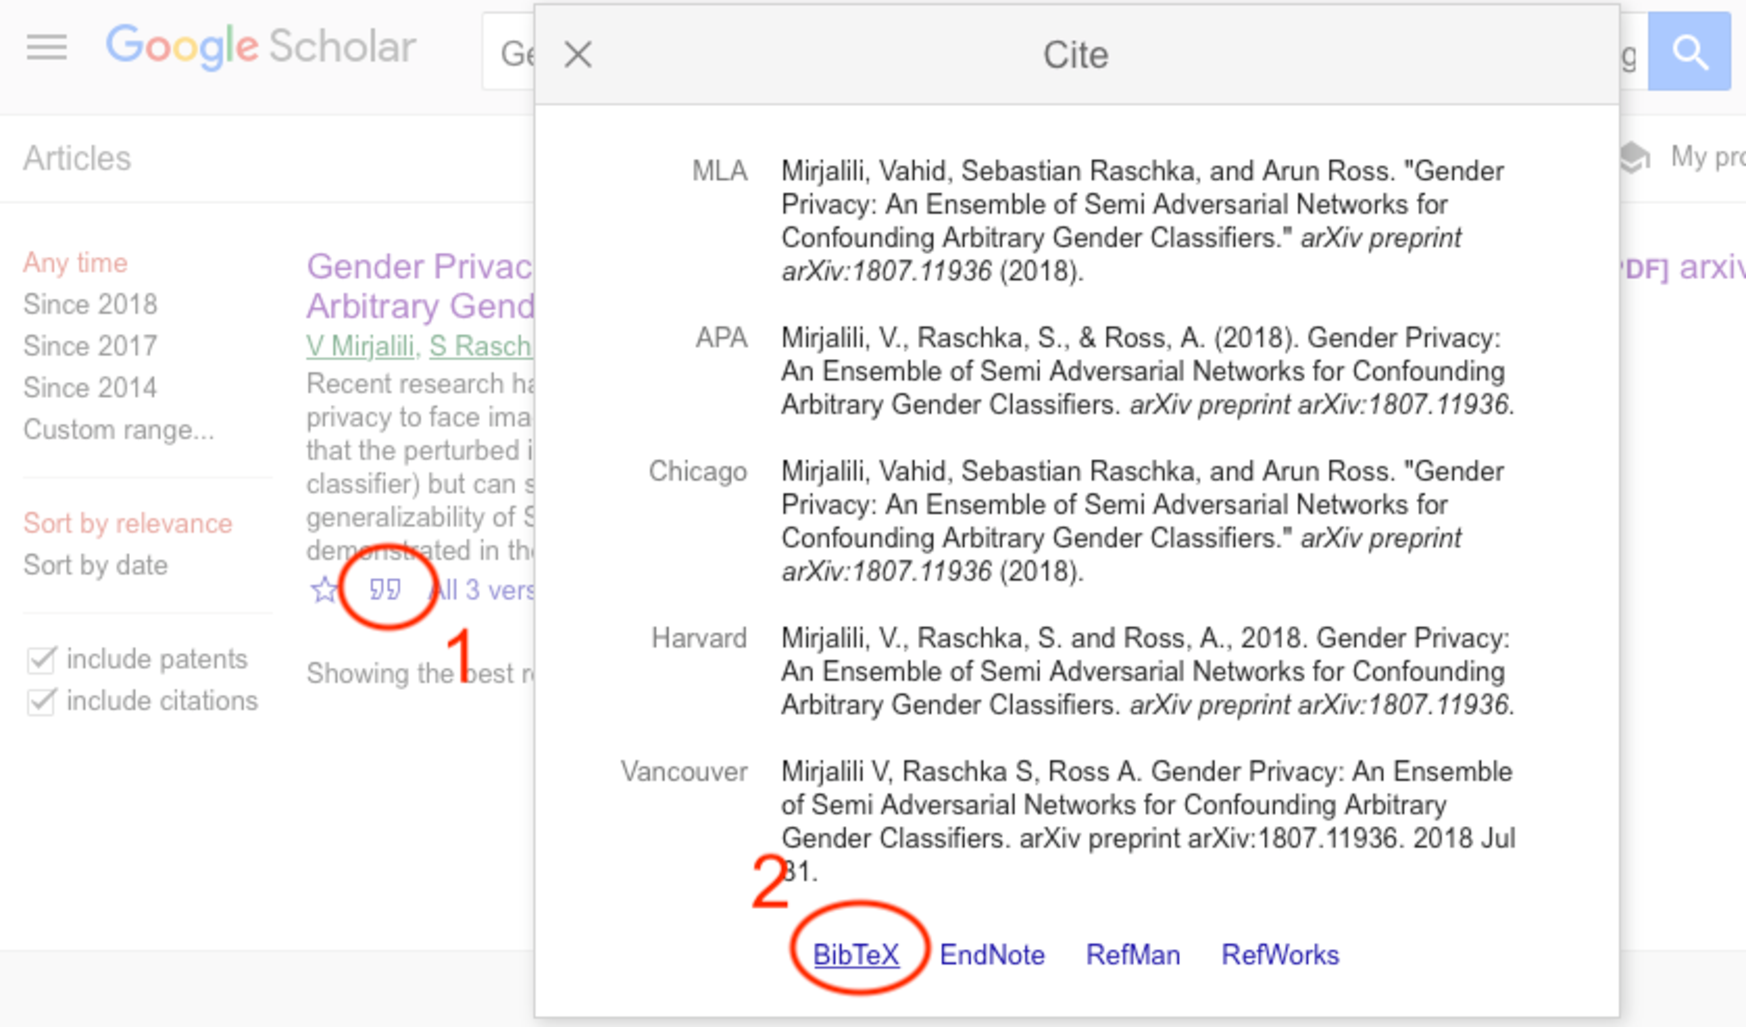
\includegraphics[width=0.8\linewidth]{figures/google-scholar.pdf}
\end{center}
   \caption{Example illustrating how to get BibTeX references from
   Google Scholar as a 1-column figure.}
\label{fig:google-scholar-1col}
\end{figure}


\begin{figure*}
\begin{center}
   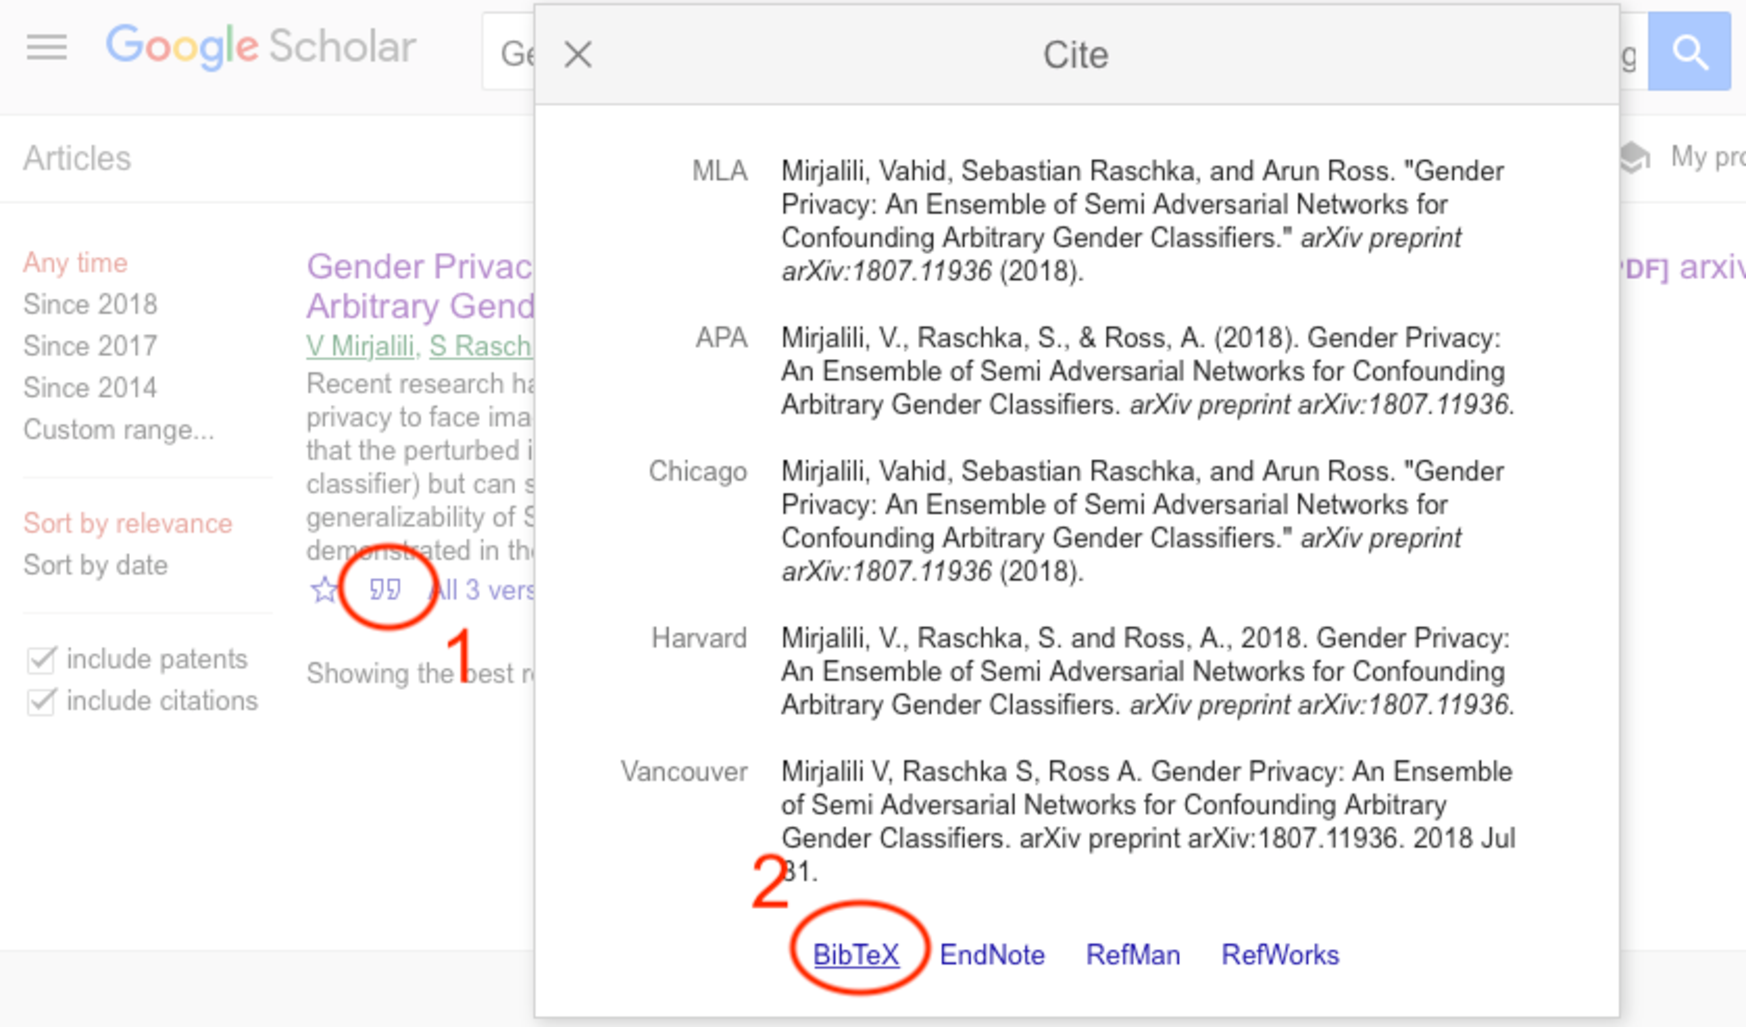
\includegraphics[width=0.8\linewidth]{figures/google-scholar.pdf}
\end{center}
   \caption{Example illustrating how to get BibTeX references from
   Google Scholar as a 2-column figure.}
\label{fig:google-scholar-2col}
\end{figure*}

Table \ref{tab:some-table} shows an example for formatting a table.

\begin{table}
\begin{center}
\begin{tabular}{|l|c|}
\hline
Method & Accuracy \\
\hline\hline
Method 1 & $70 \pm 3$ \% \\
 Method 2 & $76 \pm 3$ \% \\
\hline
\end{tabular}
\end{center}
\label{tab:some-table}
\caption{This is an example of a table.}
\end{table}


\section{Proposed Method}

Describe the method(s) you are proposing, developing, or using. I.e., details
of the algorithms may be included here. 

\section{Experiments}

Describe the experiments you performed. You may want to create separate
subsections to further structure this section.

\subsection{Dataset}

Briefly describe your dataset in a separate subsection.


\subsection{Software}

Briefly list (and cite) software software you used.

\subsection{Hardware}

If relevant, list hardware resources you used.


\section{Results and Discussion}

Describe the results you obtained from the experiments and interpret them.
Optionally, you could split "Results and Discussion" into two separate
sections.

\section{Conclusions}

Describe your conclusions here. If there are any future directions, you can
describe them here, or you can create a new section for future directions.

\section{Acknowledgements}

List acknowledgements if any. For example, if someone provided you a dataset, or
you used someone else's resources, this is a good place to acknowledge
the help or support you received.

\section{Contributions}

Describe the contributions of each team member who worked on this project.


{\small
\bibliographystyle{ieee}
\bibliography{bibliography.bib}
}

\end{document}
